%%% File: /inputs/parts/BASAL_GANGLIA_MOTOR.tex

%%% %%%%%%%%%%%%%%%%%%%%%%%%%%%%%%%%% BEGIN BASAL GANGLIA %%%%%%%%%%%%%%%%%%%%%%%%%%

There is a long history of neuroscientists constructing computational models of human cognition~\cite{McClelland79,McClellandandRumelhartPR-88,LebiereandAndersonCSS-93,OReillySCIENCE-06,BotvinickPTRS_B-07}. Different modeling tools make different assumptions and support different levels of detail from rule-based systems to spiking neurons~\cite{OReillyetalLEABRA-16,OReillyetalCCN-12,RasmussenetalPLoS-ONE-17,Eliasmith2013,BlouwandEliasmithCSS-13,JilketalJETAI-08}. In this paper, we are primarily concerned with computational models that leverage ideas from neuroscience to develop AI systems for practical problems. In this subsection and the next, we take a closer look at the basal ganglia and hippocampus using models from neuroscience that reveal computational principles we can apply in a wide range of practical problems.

%%% In this section, we consider the biological basis for action selection and higher order executive control in human beings. In particular we looks at the neural circuits generally considered to be our best guess about how reinforcement learning in implemented in the brain. These circuits assist in formulating and carrying out plans to achieve our goals and solving complex problems that require a high degree of attention, the capacity to hold several concepts in mind at a time and the ability to think about how these concepts relate to one another so as to draw new conclusions. 

%%% In each case, we start with a simplified introduction to the relevant anatomy, followed by an explanation of how the biological networks support the target capability. Later, we provide an example artificial neural network that supports a related, if not precisely equivalent capability. The two capabilities that we consider are also noteworthy for the fact that each relies upon subcortical regions that every mammal comes equipped with.  However, these functional areas have evolved considerably in humans over the last few million years as they have adapted to take advantage of and support the extended capabilities of the mammalian human neocortex.

In contrast with the relative simplicity of the neocortical architecture, the {\it{basal ganglia}} consist of specialized subcortical nuclei that are related by their evolved function. In the following, we emphasize and simplify some of those nuclei and ignore others to focus the discussion and simplify the biology. The basal ganglia provide the basis for motor activity controlled by circuits in the brainstem and conserved throughout vertebrate evolution for nearly half a billion years. The cerebral cortex has been around in the form of a six-layer sheet tiled with a repeating columnar structure since the early mammals came on the scene in the Jurassic period about 200 million years ago. Our lineage separated from mice around 100 million and from macaques and other old world monkeys around 25 million years ago. The modern human neocortex owes much to these earlier evolutionary innovations but is different in ways that make possible our facility with language, complex social organization and sophisticated abstract thinking. Compared with the basal ganglia, the neocortex is structurally elegant and functionally general.

The basal ganglia have evolved along with our neocortex to provide us with a powerful thinking machine, while at the same time leaving us to make do with some less-than-ideal adaptations. We can simulate a conventional computer in our heads but are limited to fewer than a dozen memory registers. Most of us can't perform long division in our heads even though we might know the algorithm and aided with paper and pencil carry out the necessary computations to produce an answer. We rely on the same basic cognitive machinery we use to list a few names in alphabetical order to perform all sorts of more complicated cognitive tasks. Even simpler, however, is the basic operation of choosing one of several actions to perform next. The basal ganglia play a key role in supporting action selection and it is worth looking at in a little more detail in order get a handle on some of the parts of the brain that figure prominently in human cognition. Recall that the cortex is a sheet of neural tissue more or less homogeneous in terms of its local structure quite unlike almost any other part of the brain except for the cerebellar cortex. The cortex sits on top of a structure called the {\it{thalamus}} which among other things serves as a relay in passing information back and forth between the cortex and various subcortical nuclei.

The basal ganglia consist of a bunch of circuits, of varied size, sometimes but not always consisting primarily of one cell type, sometimes but not necessarily compactly clustered together, sporting projections that seem to wander off aimlessly, but more or less located above the brainstem and below the cortex. As a general principle, if a signal sets off along some path exiting from a circuit, then expect some derivative of that signal to appear later reentering the circuit to serve as feedback. Everything about the brain, and your entire body for that matter, has to be carefully regulated to maintain a dynamic state of equilibrium, and unlike human designs, evolution is generally not able to cleanly separate the parts of the circuit that perform computations in service to behavior from those that deal with respiration, immune response, waste removal, cell repair, death and regeneration, etc. 

%%% %%%%%%%%%%%%%%%%%%%%%%%%%%%%%%%%%%%%%%%%%%%%%%%%%%%%%%%%%%%%%%%%%%%%%%%%%%%%

%%% Figure~{\urlh{#fig_Basal_Ganglia_Anatomy_and_Physiology}{\ref{fig_basal}}}
\begin{figure}
%
  \begin{center}
%    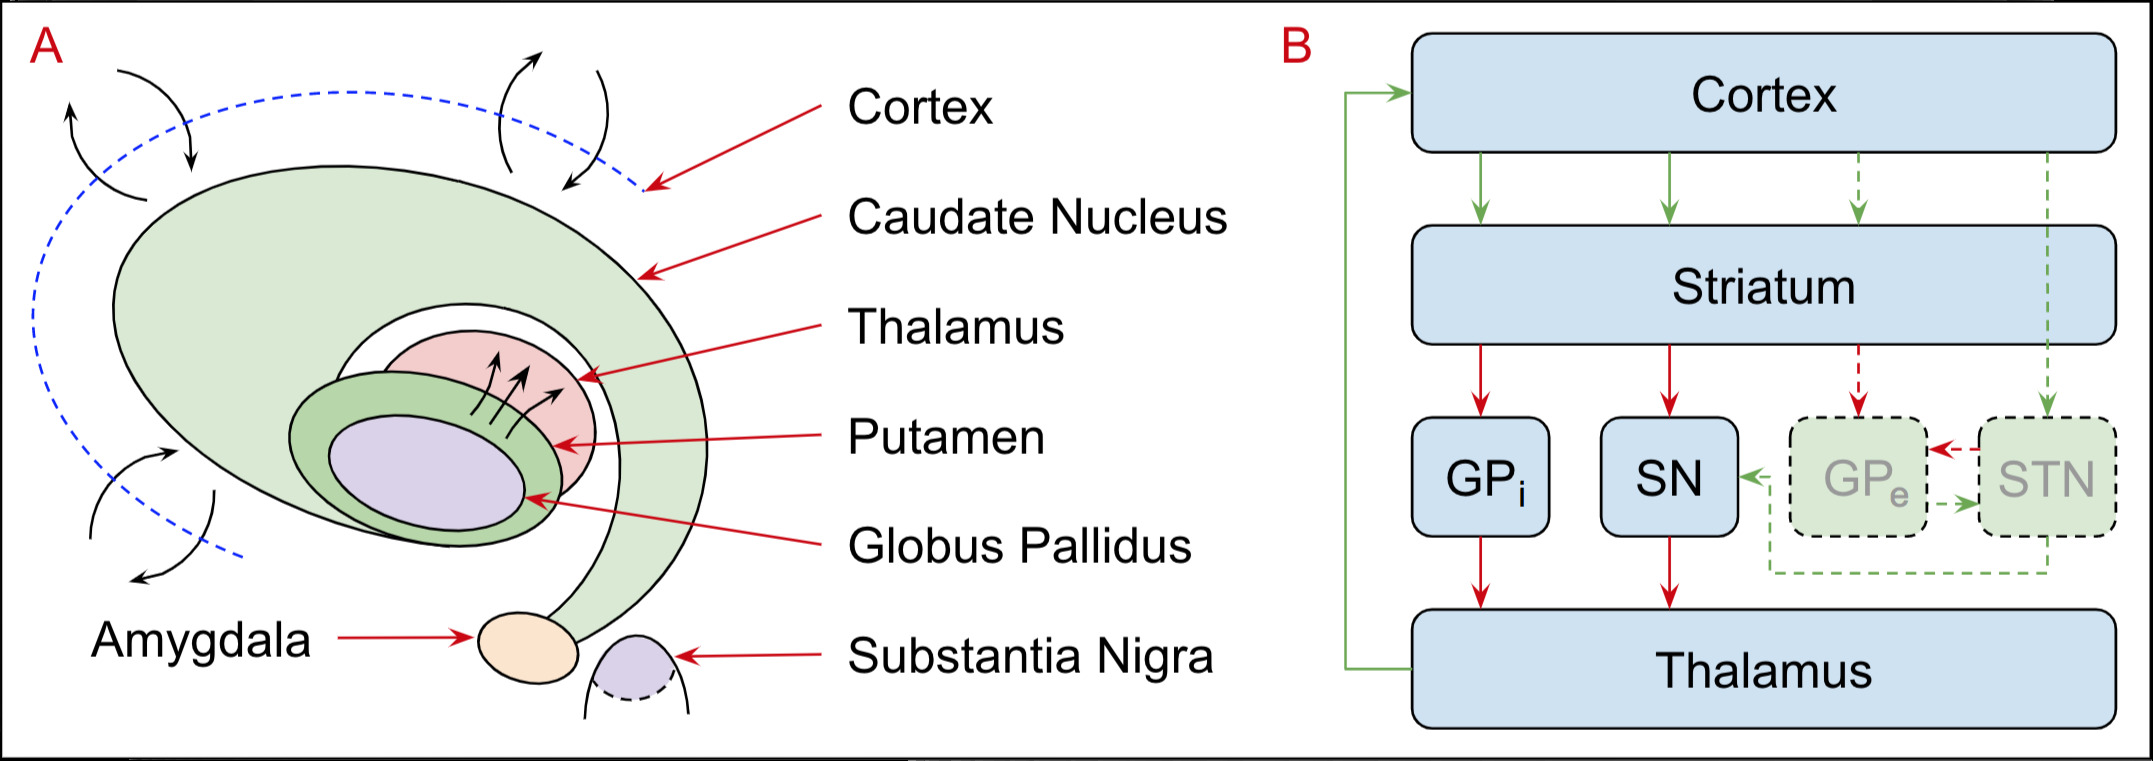
\includegraphics[width=9.0in]{./figures/Basal_Ganglia_Anatomy_and_Physiology.png} %%% 2194 × 803 pixels @ 72 per inch
    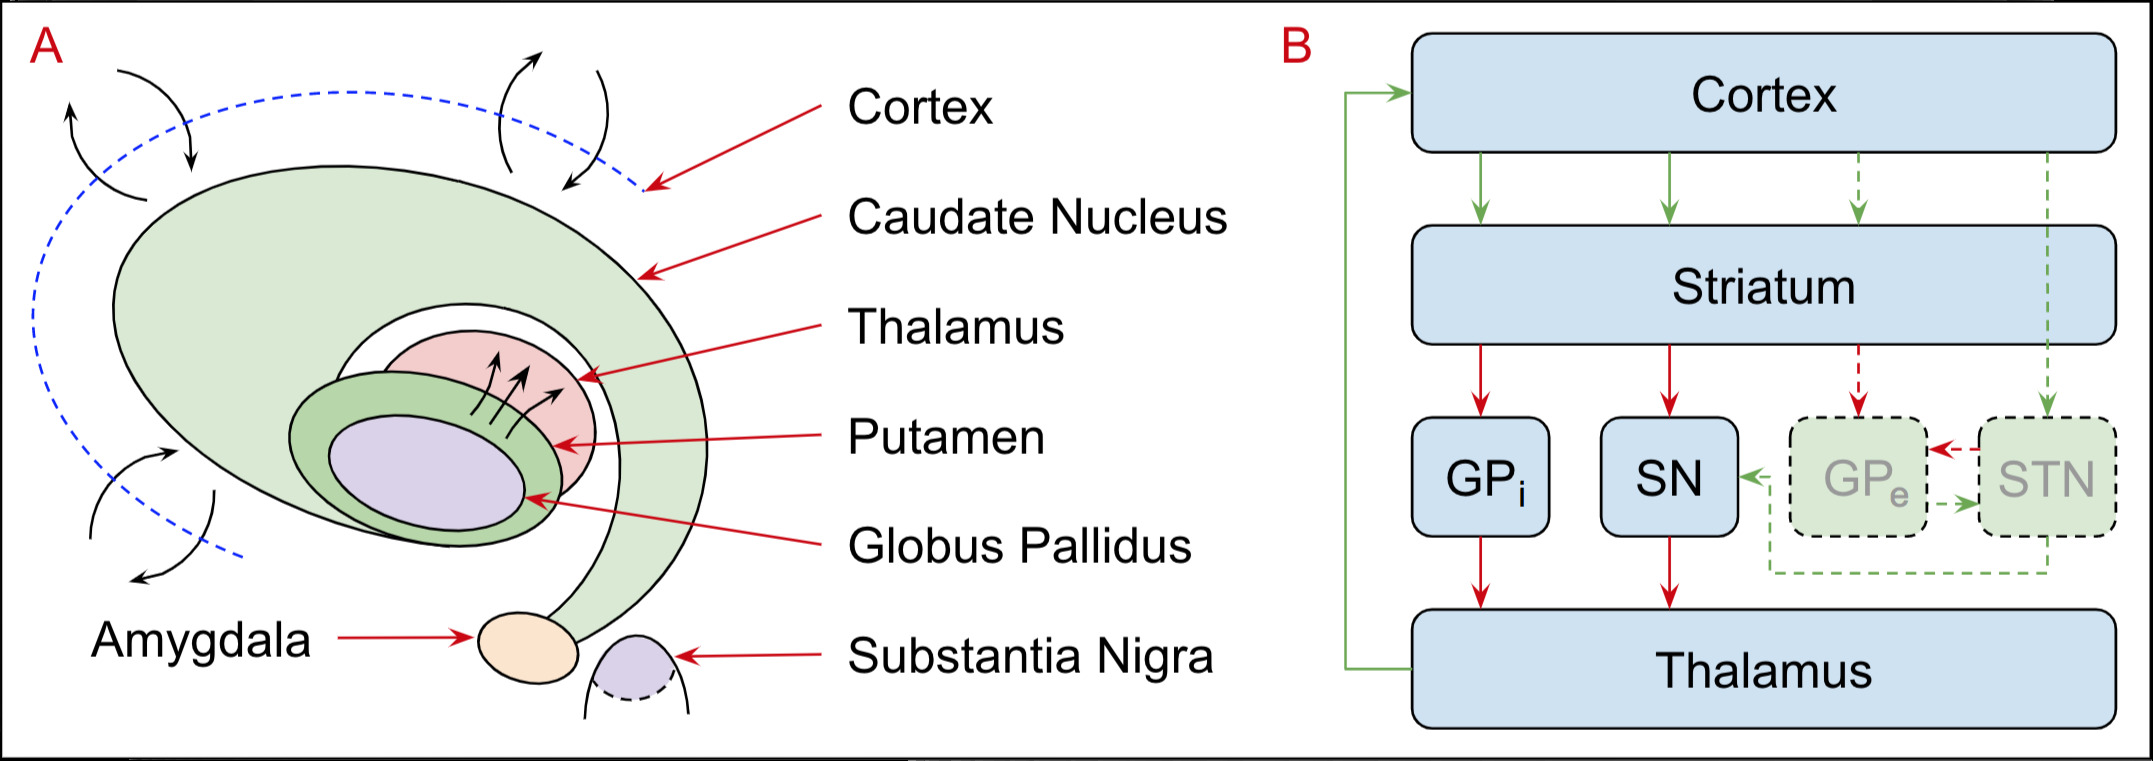
\includegraphics[width=4.0in]{./figures/Basal_Ganglia_Anatomy_and_Physiology.png} %%% 2194 × 803 pixels @ 72 per inch
  \end{center}
%
  \caption{The left panel ({\colorred{A}}) provides a highly stylized anatomical drawing of the basal ganglia. Figure~\ref{fig_broadman} ({\colorred{A}}) provides more anatomical detail while the above drawing abstracts from the structural detail in order to simplify the functional account. The block diagram shown in the right panel ({\colorred{B}}) depicts the primary components involved in action selection as functional blocks. The blocks shown in blue represent components in the {\it{direct path}} and are described in the text proper. The blocks shown in light green with dashed borders represent additional components that contribute to the {\it{indirect path}}. Good explanations of the indirect path are described in O'Reilly~\etal{}~\cite{OReillyetalCCN-12} or Wang~\etal{}~\cite{WangetalNATURE-NEUROSCIENCE-18} and we return to the basal ganglia in the next section when we look at the executive role of the prefrontal cortex in modulating behavior.}
%
  \label{fig_basal}
%
\end{figure}

%%% %%%%%%%%%%%%%%%%%%%%%%%%%%%%%%%%%%%%%%%%%%%%%%%%%%%%%%%%%%%%%%%%%%%%%%%%%%%%

The basal ganglia are depicted in Figure~{\urlh{#fig_Basal_Ganglia_Anatomy_and_Physiology}{\ref{fig_basal}}} ({\colorred{A}}) taking some artistic license to keep things simple. The thalamus along with another structure called the {\it{striatum}} provide the interface between the cortex and basal ganglia. The striatum is a combination of a number of smaller nuclei that are anatomically and functionally related; they include the Globus Pallidus (GP), Putamen and Caudate Nucleus and aside from their function as part of the striatum, only the GP will figure prominently in our discussion and only one part of it \emdash{} referred to as the {\it{internal}} GP and identified with the "i" subscript to distinguish it from the {\it{external}} part with "e" subscript.

The other players include the Substantia Nigra (SN) which is at one end of the striatum nestled close to the {\it{amygdala}} which is part of the limbic system involved with memory, decision-making and modulating emotional responses, and the Subthalamic Nucleus (STN). You can think of the cortex as integrating sensory and motor information and making suggestions for what action to take next and the amygdala as supplying information pertaining to the possible emotional consequences of taking different actions to be used as input to action selection. Figure~{\urlh{#fig_Basal_Ganglia_Anatomy_and_Physiology}{\ref{fig_basal}}} ({\colorred{B}}) reconfigures these component nuclei into a smaller number of functionally motivated blocks that control two pathways \emdash{} the {\it{direct pathway}} associated primarily with inhibition and consisting of the internal GP and SN and the {\it{indirect pathway}} playing an excitatory role and consisting of the external GP and STN~\cite{OReillyetalCCN-12,WangetalNATURE-NEUROSCIENCE-18},

The lines connecting the functional blocks shown in Figure~{\urlh{#fig_Basal_Ganglia_Anatomy_and_Physiology}{\ref{fig_basal}}} ({\colorred{B}}) imply neural connectivity, with arrows indicating the direction of influence and colors indicating the valence of the influence, green for excitatory and red for inhibitory. In the action selection cycle, the cortex forwards activations that you can think of as suggestions for what action to take next. These suggestions are propagated through the striatum and forwarded along the direct pathway where two stages of inhibitory neurons initially suppress all of the suggestions and propagate signals back the cortex to activate inhibitory neurons that suppress activity at the source. As this cycle continues, an additional process takes place in the indirect path \emdash{} identified with dashed lines \emdash{} that weighs the advantages and disadvantages of the proposed actions taking in information from throughout the cortex and adjusting the inhibitory bias accordingly.

Eventually, one proposal wins out and all of the others are suppressed allowing a single preferred action to be executed. This cycle of exploring the options for acting and then selecting a single action to execute is constantly repeated during your waking hours. Additional machinery in the thalamus and brain stem regulate whether or not to forward suggestions for acting during sleep when your cortex receives no sensory input and hence any suggestions for acting uninformed by sensory input are ill-advised if not outright dangerous. The above description doesn't begin to convey the complexity of what's going on at the level of individual neurons. Suffice it to say that the usual perfunctory summary consisting of "the winner takes all" doesn't begin to do it justice. The subtleties that arise from the way in which the evidence for and against an action proposal is combined, how ties are broken and deciding when enough evaluation is determined sufficient to make a final choice. 

%%% %%%%%%%%%%%%%%%%%%%%%%%%%%%%%%%%%% END BASAL GANGLIA %%%%%%%%%%%%%%%%%%%%%%%%%%%
